\begin{table*}[htbp]
\centering
\renewcommand{\arraystretch}{1.5}
\caption{List of articles.}
\label{table_articles}
\begin{tabular}{l@{\hspace{4em}}l@{\hspace{4em}}l@{\hspace{4em}}l@{\hspace{4em}}l}
\hline
Identifier & Study                                                                                                                                                      & Year & Publisher     & Type              \\ \hline
A01 & Gribaudo et al~\cite{Gribaudo2018} & 2018 & ScienceDirect & Journal \\
A02 & Kiss et al~\cite{Kiss2017} & 2017 & ScienceDirect & Newspaper Article \\
A03 & Pérez et al~\cite{Perez2018} & 2018 & ScienceDirect & Journal \\
A04 & Khomh et al~\cite{Khomh2018} & 2018 & ScienceDirect & Journal \\
A05 & Do et al~\cite{Do2017} & 2017 & IEEE & Conference \\
A06 & Kookarinrat et al~\cite{Kookarinrat2016} & 2016 & IEEE & Conference        \\
A07 & Zhang et al~\cite{Zhang2017} & 2017 & IEEE          & Newspaper Article \\
A08 & Lloyd et al~\cite{Lloyd2018} & 2018 & IEEE          & Journal           \\
A09 & Khazaei et al~\cite{Khazaei2017} & 2017 & IEEE          & Conference        \\
A10 & Klock et al~\cite{Klock2017} & 2017 & IEEE          & Conference        \\
A11 & Ueda et al~\cite{Ueda2016} & 2016 & IEEE          & Conference        \\
A12 & Patros et al~\cite{Patros2017} & 2017 & ACM           & Conference        \\
A13 & Alipour and Liu~\cite{Alipour2017} & 2017 & IEEE          & Conference        \\
A14 & Florio and Di Nitto~\cite{Florio2016} & 2016 & IEEE          & Conference        \\
A15 & Villamizar et al~\cite{Villamizar2015} & 2015 & IEEE          & Journal           \\
A16 & Shah et al~\cite{Shah2017} & 2017 & IEEE          & Journal           \\
A17 & Zhang et al~\cite{Zhang2017} & 2017 & IEEE          & Conference        \\
A18 & Moradi et al~\cite{Moradi2017} & 2017 & IEEE          & Conference        \\
A19 & Casalicchio and Perciballi~\cite{Casalicchio2017} & 2017 & IEEE          & Conference        \\
A20 & Toffetti et al~\cite{Toffetti2015} & 2015 & ACM           & Conference        \\
A21 & Julian et al~\cite{Julian2016} & 2016 & ACM           & Journal           \\
A22 & Suresh et al~\cite{Suresh2017} & 2017 & ACM           & Journal           \\
A23 & Khazaei et al~\cite{Khazaei2017} & 2017 & ACM           & Journal           \\
A24 & Barna et al~\cite{Barna2017} & 2017 & IEEE          & Conference        \\
A25 & Ben Hadj Yahia et al~\cite{BenHadjYahia2016} & 2016 & ACM           & Conference        \\
A26 & Gotin et al~\cite{Gotin2018} & 2018 & ACM           & Conference        \\
A27 & Klinaku et al~\cite{Klinaku2018} & 2018 & ACM           & Conference        \\
A28 & López et al~\cite{Lopez2017} & 2017 & ACM           & Conference        \\
A29 & Jenkins et al~\cite{Jenkins2017} & 2017 & IEEE & Conference        \\
A30 & Salah et al~\cite{Salah2017} & 2017 & IEEE          & Conference        \\
A31 & Singh et al~\cite{Singh2017} & 2017 & IEEE          & Conference        \\
A32 & Amaral et al~\cite{Amaral2016} & 2016 & IEEE          & Journal           \\
A33 & Al-Dhuraibi et al~\cite{Al-Dhuraibi2017} & 2017 & IEEE          & Journal           \\
A34 & Benchara et al~\cite{Benchara2017} & 2017 & IEEE          & Conference        \\ 
A35 & Higashino~\cite{Higashino2017ApplicationArchitecture} & 2017 & ACM          & Journal        \\ \hline
\end{tabular}
\end{table*}

In this section, we present the results obtained from the 35 fully assessed studies related to the research topic. We attempt to answer each proposed research question in the following subsections through elaborative information synthesis. After answering the research questions, we created an updated taxonomy with the state-of-the-art of applications microservice and how to improve scalability and performance. 

\subsection{Conducting the Search Strategy}
We selected 4 electronic databases as our search scope. We used ACM Digital Library, IEEE Xplore Library, ScienceDirect, and SciELO. These portals cover the most relevant journals and conferences within computer science. In the next subsection, we explain how we filter the studies. Figure~\ref{article_selection} shows our filtering process. 

\begin{figure*}[htb]
\centering
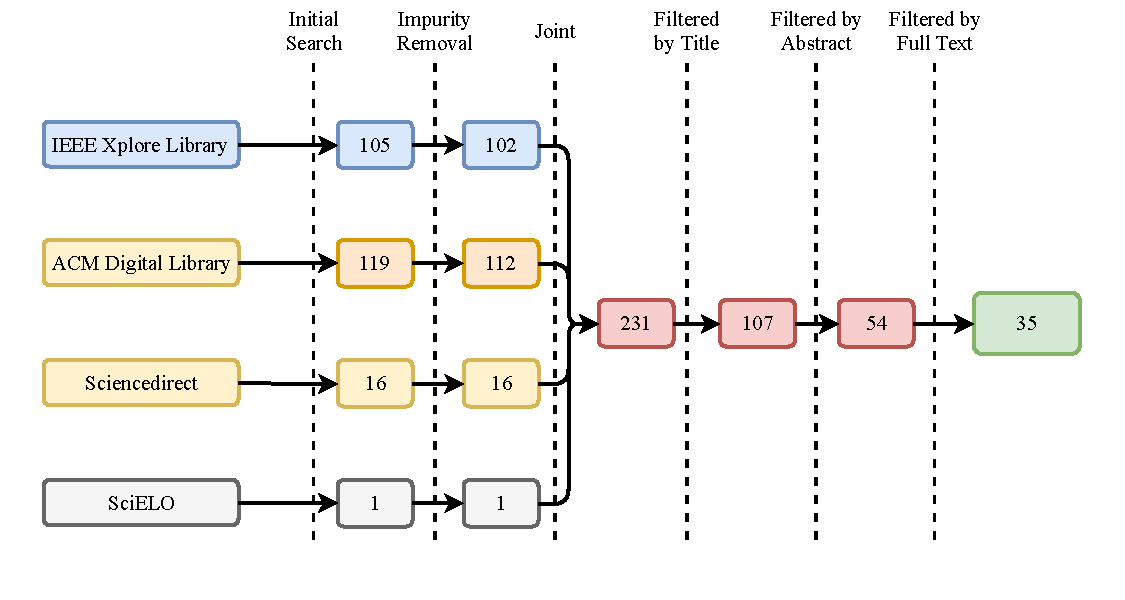
\includegraphics[scale=0.7]{Images/Article_selection.pdf}
\caption{Systematic mapping study - article selection.}
\label{article_selection}
\end{figure*}

We found 241 articles in the initial search before applying the exclusion criteria. After that, we performed the impurity removal that removes 10 (4.15\%) articles. Then, we joint the articles resulting in 231 articles. So, we filtered by title resulting in 107 (46.32\%) articles. Continuing the process, we perform a filter in abstract resulting in 54 (50.47\%) articles. Finally, we apply the exclusions criterion in the full text remained 35 (64.81\%) articles. These articles are the baseline for the study. Table~\ref{table_articles} shows an overview of all primary studies with the identifier, reference, publication year, publisher, and type.

\begin{figure*}[h!bt]
\centering
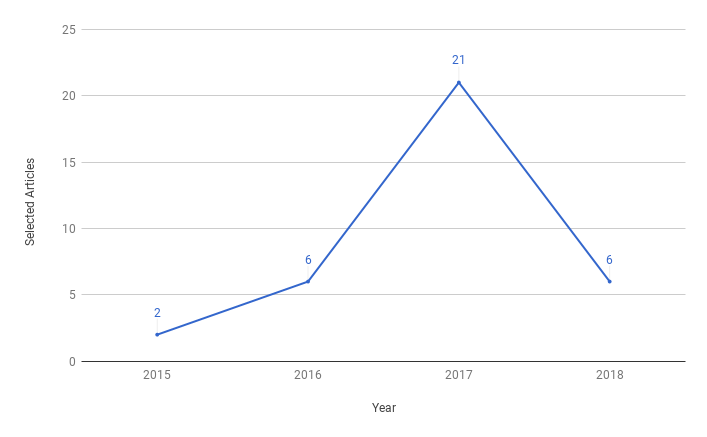
\includegraphics[scale=0.5]{Images/publication_chronology.png}
\caption{Publication chronology.}
\label{chronology}
\end{figure*}

In Figure~\ref{chronology}, we present the evolution of the selected publications over the years, covering from 2015 to 2018. This figure shows that we find recent articles in our research demonstrating that microservice is a new trend.

\begin{figure*}[htb]
\centering
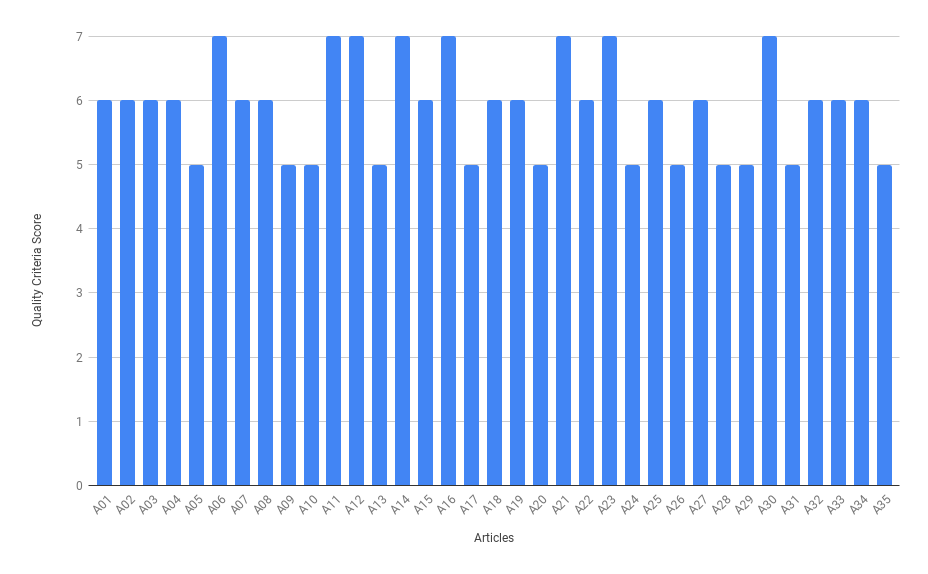
\includegraphics[scale=0.40]{Images/Quality_chart.png}
\caption{Quality assessment of the articles.}
\label{quality_chart}
\end{figure*}

\subsection{Performing the Quality Assessment}
In Figure~\ref{quality_chart}, we show the quality criteria score of the articles based on the quality assessment criteria proposed in Table~\ref{table_questions}. The quality criteria score for each article obtained is shown on the vertical axis and the studies themselves on the horizontal axis, from 1 to 35. This figure demonstrated that the articles responded positively to at least 5 out of 7 quality assessment criteria. For instance, several articles do not comment on or cite possible future studies in general because they are conclusive articles, with a conclusion on its assessment. Besides, some articles do not address the literature review, background, or context, because they are technical articles.

\subsection{Answers to the Research Questions}

Finally, to address the general and specific research questions, we have identified the following.

\subsubsection{CG1 How would the microservice performance and scalability appear?}
\begin{table*}[!bt]
\centering
\renewcommand{\arraystretch}{1.5}
\caption{Properties of microservice performance and scalability in articles.}
\label{table_CG1}
\begin{tabular}{ll@{\hspace{8em}}l}
\hline
\multicolumn{2}{l}{Group and item} & Description \\ \hline

\multicolumn{2}{l}{\textbf{Evaluation}} &  \\
 & Metrics & Metrics used to evaluate the performance and scalability (see subsection SQ1) \\
 & Algorithm & Algorithms to evaluate performance and scalability (see subsection SQ1) \\
 
\multicolumn{2}{l}{\textbf{User Application}} &  \\
 & Application classes & Application types of microservices (see subsection SQ2) \\
 
\multicolumn{2}{l}{\textbf{Architectures}} &  \\
 & Distributed system & Describes the main architecture models (see subsection SQ3) \\
 & Virtualization & Describes the virtualization type of microservices (see subsection SQ3) \\
 
\multicolumn{2}{l}{\textbf{Communication}} &  \\
 & Patterns & Communication patterns of microservices (see subsection SQ4) \\
 & Protocol & Communication protocol of microservices (see subsection SQ4) \\ \hline
\end{tabular}
\end{table*}
We search characteristics of microservice performance and scalability in articles. We want to find metrics, patterns, protocols, architecture and applications classes of microservice. We review the selected articles to find these characteristics. Table~\ref{table_CG1} presents the results for this review. This table leads the remains research questions.

We used this classification to build the taxonomy (present in section taxonomy). We believe that this taxonomy could help to classify, compare, and evaluate different architectures and solutions for microservices. Table~\ref{table_CG1} presents four groups: (1) Evaluation, (2) User Application, (3) Architectures, and (4) Communication. Each item from the table has a brief description of the classification. Furthermore, the items have a binding with the specific research question that explores the item.

\subsubsection{CG2 What are the motivations for analyzing and improving microservice?}
\begin{table*}[tb]
\centering
\renewcommand{\arraystretch}{1.5}
\caption{Motivations to analyze and improve microservice.}
\label{table_CG2}
\begin{tabular}{llll}
\hline
\multicolumn{2}{l}{Group and identifier} & Description & Reference articles \\ \hline

\multicolumn{2}{l}{\textbf{Metric analysis}} &  &  \\
 & Energy & Analysis of the energy consumption of microservices & A01, A04 \\
 & Cost & Evaluate the microservice application cost & A01, A03, A08, A09, A13, A15, A28 \\
 &  &  & A31 \\
 & Performance & Analysis of the microservice performance & A01, A03, A04, A05, A06, A07, A08, \\
 &  &  & A09, A10, A11, A12, A13, A14, A15, \\
 &  &  & A16, A17, A18, A19, A20, A21, A22, \\
 &  &  & A23, A24, A25, A26, A27, A29, A30, \\
 &  &  & A31, A32, A33, A34, A35 \\
 & Reliability & Analysis of the reliability of the microservice application & A04, A12, A17, A23, A26 \\
 
 \multicolumn{2}{l}{\textbf{Deployment}} &  &  \\
 & Update & Evaluate the impact of microservice update on performance & A15, A24, A31 \\
 
 \multicolumn{2}{l}{\textbf{Architecture}} &  &  \\
 & Communication & Analysis of the communication impact in performance & A06 \\
 & Scalability & Evaluate the scalability of the microservice architecture & A01, A02, A04, A05, A06, A07, A10 \\
 &  &  & A11, A18, A23, A25, A27, A28, A31 \\
 &  &  & A32 \\ \hline
\end{tabular}
\end{table*}
In this question, we want to find what are the motivations from the articles to analyze the microservice behavior. The major contribution of this question is presents the common concerns in microservice performance and scalability aspects. 

Table~\ref{table_CG2} presents the result from our research on this question. This table has three groups to describe the concerns in microservice related to metric analysis, deployment, and architecture. 
The metric analysis group aims to answer why is necessary to analyze metrics in a microservice environment, ranging from performance investigation to measure the reliability of the system. Besides that, another interest involves examination of microservice cost, particularly interesting in public clouds, and metrics to analyze the energy consumption.

The second group is the deployment that a investigate the impact of microservice update on the performance and scalability. With DevOps, programmers continually modify the microservice source-code, so it is difficult to know the right moment to deploy some modification.

Finally, the Architecture group analyze the concerns when a developer wants to create a microservice architecture, like how to guarantee the system scalability and how to implement the communication between microservices.

\subsubsection{SQ1 Which are the metrics and algorithms used to evaluate microservice?}
\begin{table*}[p]
\centering
\renewcommand{\arraystretch}{1.5}
\caption{Types and metrics used to evaluate microservice behavior.}
\label{table_SG1}
\begin{tabular}{llll}
\hline
\multicolumn{2}{l}{Group and identifier} & Description & Reference articles \\ \hline

\multicolumn{2}{l}{\textbf{Metrics}} &  &  \\
 & CPU & Percentage of CPU utilization & A02, A06, A08, A09, A13, A14, A16, \\
 &  &  & A17, A19, A20, A23, A24, A26, A30, \\
 &  &  & A32, A33 \\
 & Memory & Memory consumption & A06, A08, A16, A17, A20, A23, A33 \\
 & Execution time & Application execution time or response time & A01, A03, A04, A05, A07, A08, A10, \\
 &  &  & A12, A15, A19, A20, A24, A25, A28, \\
 &  &  & A29, A30, A31, A34 \\
 & Task queue & Length of task queue & A05, A20, A25, A26, A27 \\
 & Network throughput & The network throughput between the microservices & A06, A11, A16, A17, A18, A21,\\
 &  &  & A22, A23, A32 \\
 & Task processing rate & Number of tasks processed per time & A01, A10, A12, A20, A24, A30, \\
 &  &  & A31 \\
 
 \multicolumn{2}{l}{\textbf{Types}} &  &  \\
 & Relative & The share that each container has of the resources used & A01, A02, A03, A04, A05, A06, A07, \\
 &  &  & A08, A09, A10, A11, A12, A13, A14, \\
 &  &  & A15, A16, A17, A18, A20, A21, A22, \\
 &  &  & A23, A24, A25, A26, A27, A28, A29, \\
 &  &  & A30, A31, A32, A33, A34 \\
 & Absolute & Actual utilization of host system resources & A19 \\
 
\multicolumn{2}{l}{\textbf{Algorithm}} &  &  \\
 & Reactive & Perform decisions when reaches a threshold & A02, A05, A07, A09, A14, A19, A20, \\
 &  &  & A23, A24, A25, A26, A27, A33 \\
 & Proactive & Perform decisions proactively, before reach a threshold & A01, A12, A13, A16, A17 \\
 
\multicolumn{2}{l}{\textbf{Proactive algorithm}} &  &  \\
 & Pattern analysis & Analyze application patterns to improve performance & A01, A17 \\
 & Mathematical model & Use mathematical models to analyze the behavior & A12, A17 \\
 & Machine learning & Use machine learning to analyze the behavior & A13, A16 \\ \hline
\end{tabular}
\end{table*}
To answer this research question, we analyzed all selected studies that involved research of the metrics and algorithms used in microservice evaluation. Table~\ref{table_SG1} summarized the results of this analysis. We divided this table into four groups.

The first group presents the metrics found in the studies. We found both metrics of host health, like CPU and memory, and application status, like execution time and task queue.

Another group is the metrics types used to evaluate the application. We associated this group with metrics that show the host health such as CPU and memory. There are two types of metrics: (1) Relative metrics and (2) Absolute metrics. In Relative metrics, the value of a metric is just the portion that the host allocates to container/virtual machine. In Absolute metrics, the value is the actual utilization of host resources.

After dividing the metrics, we show the algorithms to evaluate these metrics and perform actions. We found two types of algorithms: (1) Reactive and (2) Proactive. In the reactive form, the system performs an action when a threshold reaches. Already in Proactive form, the system predicts an action before a threshold reaches.

Finally, the last group divides the Proactive form in the algorithms to predicts the application behavior. We found three types: (1) Pattern analysis which matches the application behavior to a template, (2) Mathematical model which applies some mathematical model to analyze the application behavior and predicts future values, and (3) Machine learning which uses a machine learning, such as neural network, to predicts system behavior.

\subsubsection{SQ2 Which are microservice applications classes?}
\begin{table*}[tb]
\centering
\renewcommand{\arraystretch}{1.8}
\caption{Microservices applications types.}
\label{table_SG2}
\begin{tabular}{l@{\hspace{1em}}l@{\hspace{3em}}l@{\hspace{2em}}l}
\hline
\multicolumn{2}{l}{Group and identifier} & Description & Reference articles \\ \hline

\multicolumn{2}{l}{\textbf{Transactional}} &  &  \\
 & Web requests & Requests to a host, like HTTP requests & A01, A07, A11, A14, A15, A16 A24, \\
 &  &  & A25, A27, A30, A31, A33 \\
 & Streaming & Multimedia streaming, like audio/vídeo & A13, A17 \\
 & Data transfer & Data transfer of files & A02, A28 \\
 
\multicolumn{2}{l}{\textbf{Batch}} &  &  \\
 & Image Processing & Processing to transform a image & A03, A34 \\
 & Mathematical model & Computation to resolve a mathematical problem & A08, A09, A19, A32 \\
 & ERP & Enterprise Resource Planning & A10 \\
\multicolumn{2}{l}{\textbf{IoT}} & Internet of things & A23, A26 \\ \hline
\end{tabular}
\end{table*}
Now, we want to know what are the classes of the microservice application that articles used. It is crucial because each class has a different approach to evaluate and improve application performance and scalability. For example, transactional applications have a long execution time compared with a batch application. So the best algorithm to use in this type of application is different. 

Table~\ref{table_SG2} shows the classes of the application that we found in our review. We divided the application class into three main groups. The first one is the Transactional application, such as web requests, data transfer, and streaming. This type of application needs to resolve many requests to a server. 

Another type of application is the batch applications that involves image processing, mathematical model, and enterprise resource planning. Unlike the transactional application, the batch application has one request and perform processing.

The last group of application is the Internet of things applications. This class of application involves sensors that produce data. A microservice application can process the data generated by sensors to provide some useful information.

\subsubsection{SQ3 What are the distributed system architecture of microservice applications?}
\begin{table*}[tb]
\centering
\renewcommand{\arraystretch}{1.8}
\caption{Distributed system architecture of microservice applications to improve performance and scalability.}
\label{table_SG3}
\begin{tabular}{llll}
\hline
\multicolumn{2}{l}{Group and identifier} & Description & Reference articles \\ \hline

\multicolumn{2}{l}{\textbf{Architecture}} &  &  \\
 & Cache based & Use a cache to improve microservices performance. & A03, A25, A29, \\
 & Load balancer & A load balancer defines the better host to perform tasks. & A05, A06, A15, A20, A22, A24, A31 \\
 &  &  & A34 \\
 & Mobile agent & A agent migrates to each host to evaluate and adjust the system. & A35 \\
 & Cloud & Elasticity feature to improve performance. & A01, A02, A05, A07, A09, A12, A13, \\
 &  &  & A14, A17, A19, A20, A23, A24, A25, \\
 &  &  & A27, A28, A33 \\
 
\multicolumn{2}{l}{\textbf{Elasticity}} &  &  \\
 & Vertical & Increases/decreases machines/containers capacity. & A33 \\
 & Horizontal & Add and remove computer nodes. & A01, A02, A05, A07, A09, A12, A13, \\
 &  &  & A14, A17, A19, A20, A23, A24, A25, \\
 &  &  & A27, A28 \\
 
\multicolumn{2}{l}{\textbf{Virtualization}} &  &  \\
 & Virtual machines & Operating system and hardware virtualization. & A01, A05, A08, A09,  A22, A23, A24, \\
 &  &  & A30, A32, A35 \\
 & Containers & Operating system virtualization. & A02, A03, A08, A11, A14, A16, A17, \\
 &  &  & A18, A19, A21, A24, A25, A27, A28, \\
 &  &  & A30, A31, A32, A33 \\ \hline
\end{tabular}
\end{table*}
Another result was the identification of distributed system architecture used in microservice applications. The definition of a distributed system is important to improving scalability and performance. Table~\ref{table_SG3} presents these results. 

We found three types of information. The first group is the architecture used in each article. We found four architectures: (1) Cache based that involves a cache of microservices or cache of response, (2) Load balancer that defines the best host to process the requisitions, (3) Mobile agents that involve an agent that migrate between hosts and adjust the host, and (4) Cloud that we detailed in section~\ref{background}.

The second group detail how the cloud could improve performance and scalability using elasticity. Elasticity could be vertical or horizontal. We explain this in section~\ref{background}.

Finally, the last group is the virtualization to cloud computing. We divided into (1) Virtual machines and (2) Containers. We detailed this in section~\ref{background} too.

\subsubsection{SQ4 Which are communication patterns and protocols to microservice?}
\begin{table*}[tb]
\centering
\renewcommand{\arraystretch}{1.8}
\caption{Communication patterns and protocols to microservice.}
\label{table_SG4}
\begin{tabular}{llll}
\hline
\multicolumn{2}{l}{Group and identifier} & Description & Reference articles \\ \hline

\multicolumn{2}{l}{\textbf{Patterns}} &  &  \\
 & Direct & The microservices communicates directly. & A13, A17, A22, A24, A28, A30 \\
 & Gateway & Use a gateway between the microservices. & A02, A06, A11, A15, A19, A20, A29, \\
 &  &  & A31, A34 \\
 & Message BUS & Use a message BUS to communicates between microservices. &  A06, A27, A34 \\
 
\multicolumn{2}{l}{\textbf{Protocol}} &  &  \\
 & HTPP/REST & Use REST API to communicates with microservices. & A02, A04, A05, A06, A08, A09, A14,  \\
 &  &  & A16, A24, A28, A31, A33, A35 \\
 & AMQP & Application layer protocol for message-oriented middleware. & A27, A34 \\
 & RPC & Remote protocol call. & A22, A29 \\ \hline
\end{tabular}
\end{table*}
The last question involves determinating the communication patterns and protocols to deploy microservice applications. Table~\ref{table_SG4} detailed the results found.

First, we classified the communication patterns of microservice using the three types explained in section~\ref{background}: (1) Direct communication, (2) Gateway communication, and (3) Message BUS communication.

So, we divided the articles into protocols used in communication between microservices and external applications. We found three types of protocol: (1) HTTP requests using REST API, (2) AMQP protocol that implements a queue of tasks, and (3) Remote protocol call. 